\chapter{Testování}\label{kap:test}
Tato kapitola se věnuje testování nejen systému jako celku, ale i testování jednotlivých komponent. Kromě testování funkčnosti systému, je kapitola též zaměřena na zátěžové testy serverových aplikací. Do zátěžových testů patří například zjištění, do kolika jednotek jsou jednotlivé aplikace schopné zpracovávat data bez zahlcení. Další částí jsou testy programu pro balancování zatížení serverových aplikací. Ten umožňuje spuštění několika instancí TCP a UDP serveru na více zařízeních, a tím navýšit limit zpracovávaných zpráv. Kapitola je také věnovaná testování zabezpečení síťové komunikace mezi jednotkou a serverovými aplikacemi a komprimace odesílaných dat.

\section{Test instalačních skriptů a kompletní funkce systému}
Cílem tohoto testu je vyzkoušet správnou funkčnost instalačních skriptů. Při správném fungování by po přípravě microSD karty a databáze měla jednotka během pár minut bez jakéhokoliv zásahu začít měřit a naměřená data odesílat na server.

Tento test byl prováděn s~rozšiřující deskou ve verzi 1.0. Desky ve verzi 1.0 a 1.1 nedisponují unikátním identifikátorem a z~toho důvodu bylo zvoleno jako ID kombinace MAC adresy RPi a typu jednotky. Před inicializací jednotky je nutné jednotku v~databázi vytvořit a k~tomu je potřeba znát ID. Pro zjištění identifikátoru byla do RPi vložena karta s~neupravenou instalací operačního systému Raspian a spuštěn příkaz:
\begin{lstlisting}[language=bash, breaklines, label={code:uid}]
$ echo "c0$(cat /sys/class/net/eth0/address | tr -d ':' | tail -c 7)"
\end{lstlisting}
Tento příkaz na standardní výstup vypíše dvě hodnoty pro námi zvolený typ jednotky ($c0$) a posledních šest hodnot MAC adresy jednotky. V~případě testované jednotky to je $d2bdb4$. Do databáze je tedy přidána jednotka s~tímto ID. Následně jsou v~databázi vytvořeny čtyři senzory s~potřebnými parametry a pomocí programu \textit{ConfigGenerator} je vygenerován konfigurační soubor \textit{config}, jehož obsah je možné vidět na přiloženém médiu v~kořenovém adresáři. Před přidáním nové jednotky do systému musí být vytvořena i příslušná databáze v~časové databázi a uživatelským účtům musí být přidělena práva pomocí skriptu \textit{privileges.sh}. Po provedení těchto kroků je již serverová část připravena na provoz nové jednotky. Dalším krokem pro zprovoznění nové jednotky je vytvoření obrazu operačního systému Raspbian na kartě a spuštění skriptu \textit{SDCardInit.sh}. Jednotka s~připravenou kartou musí být před spuštěním připojena k~internetu pomocí ethernetového kabelu, jinak nedojde ke stažení knihoven a softwaru. Tímto je dokončena příprava na instalaci.

Jednotka s~připravenou kartou byla spuštěna v~11:48:21 a instalace byla dokončena v~12:15:15. Jednotka má nastavené dvouminutové zpoždění pro spuštění čtecích programů (zamezení restartovací smyčky způsobené možnou nestabilitou čtecího programu) a první agregované hodnoty byly tedy do databáze zapsány o~zhruba dvě až tři minuty později, viz obrázek \ref{pic:installsdf}. Na obrázku je možné vidět, že byly přijaty agregované hodnoty ze čtyř senzorů. K~jednotce nebyl připojen senzor, jedná se tedy pouze o~šum na analogovém vstupu.
\begin{figure}
  \centering
  \scalebox{0.21}{
        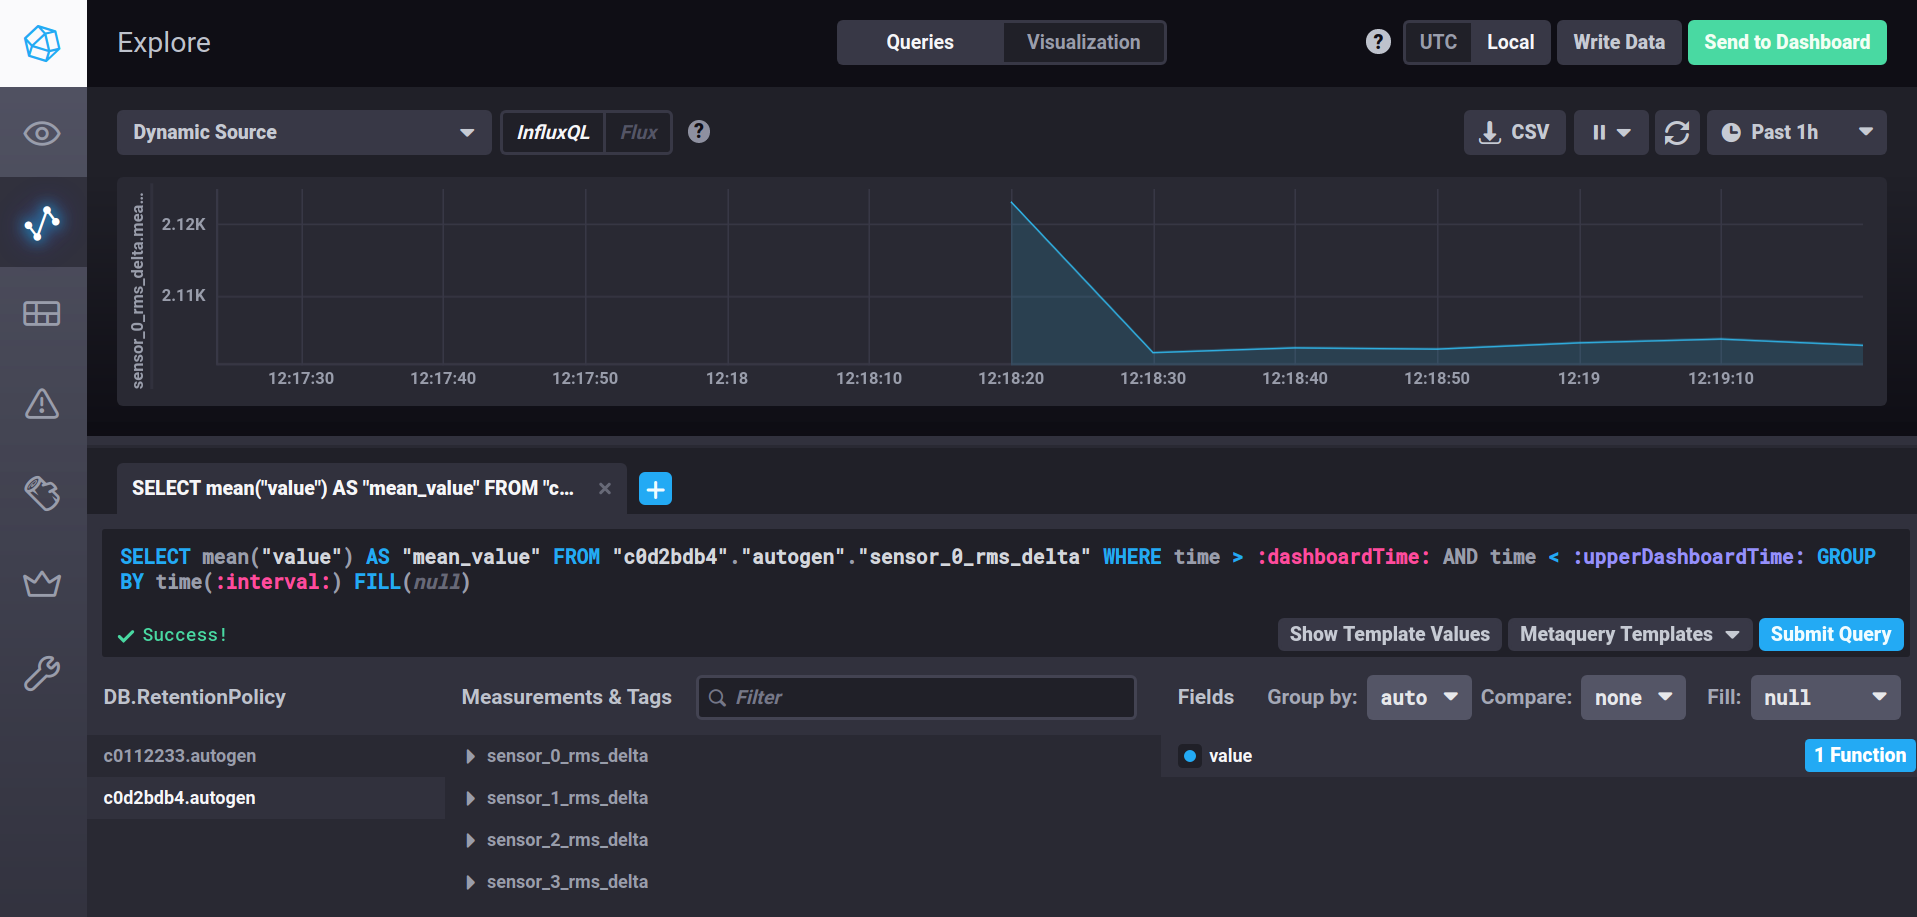
\includegraphics{obrazky-figures/influx_instal_data.png}
    }
  \caption{První přijatá data po dokončení instalace.}\label{pic:installsdf}
\end{figure}
Konfigurační soubor byl před spuštěním úspěšně stažen ze serveru. Na obrázku \ref{pic:htop} je vidět rozložení procesů na jednotlivých jádrech. Z~obrázku je patrné, že program \textit{Reader} využívá dvě procesorová jádra, která pro něj byla alokována. Proces využívající třetí jádro provádí čtení dat z~nastaveného rozhraní. Stoprocentní využití jádra způsobuje aktivní čekání na signál \textit{data ready}. Proces spuštěný na čtvrtém jádře aplikuje filtry na bloky dat získaných od čtecího procesu a využívá jádro průměrně na $50 \%$. Oba procesy mají RT prioritu. Agregační program je spuštěn na zbývajících jádrech společně se systémem.
\begin{figure}
  \centering
  \scalebox{0.30}{
        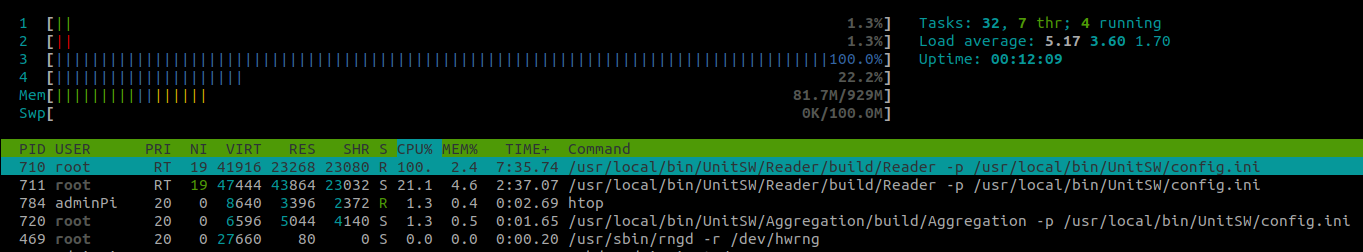
\includegraphics{obrazky-figures/htop.png}
    }
  \caption{Využití procesoru při čtení a rozložení procesů na jednotlivých jádrech.}\label{pic:htop}
\end{figure}
Soubory s~logy byly vytvořeny správně na nastavené cestě a obsahovaly informaci o~neúspěšném pokusu o~navázání TCP spojení. Při kontrole konfiguračního souboru byla objevena chyba v~IP adrese pro TCP server. IP adresa byla opravena na serveru a opravený soubor byl jednotkou během následujících pěti minut stažen a došlo k~restartování čtení a byla navázána i TCP komunikace viz obrázek \ref{pic:tcpinstall}. 
\begin{figure}
  \centering
  \scalebox{0.34}{
        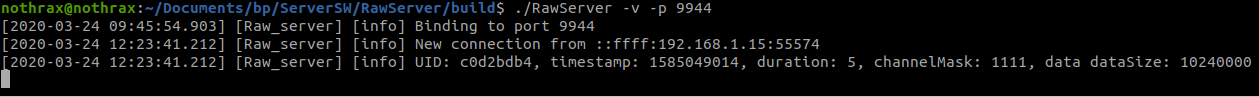
\includegraphics{obrazky-figures/raw_connection.png}
    }
  \caption{Informace o~příchozí zprávě na TCP server.}\label{pic:tcpinstall}
\end{figure}
Výstup instalačního skriptu je směřován do souboru \textit{install\_log.txt}. Tato vlastnost je důležitá pro kontrolu instalace. Pokud dojde při instalaci k~jakékoliv chybě, je možné záznam o~ní vyhledat právě v~tomto souboru. Soubor z~testovací instalace je přiložen v~kořenové složce na přiloženém médiu. Výstup skriptu byl zkontrolován a neobsahuje žádná chybová hlášení.

Tento test ověřil funkčnost bezzásahové inicializace jednotky a dobu nutnou k~jejímu zprovoznění. Čas potřebný pro zaměstnance pro přidání jednotky do databáze a přípravu instalační karty je zhruba deset minut a je zde prostor pro další urychlení. Například vytvořením jednoduchého uživatelského rozhraní, přes které by bylo možné na jednom místě jednoduše přidat jednotku do databáze a vytvořit její instalační kartu. Bezzásahová instalace jednotky trvala zhruba 27 minut a měření bylo zahájeno po 30 minutách. Tímto testem byla vyzkoušena i kompletní funkcionalita celého systému.

\section{Komprimace zpráv}
Cílem testu bylo porovnat kompresní algoritmy pro využití při odesílání neagregovaných dat a zvolit nejvhodnější algoritmus pro implementaci v~jednotce. TCP zprávy obsahující nezpracovaná data mohou nabývat velikosti až několik MB. Z~toho důvodu je vhodné využít rychlý kompresní algoritmus pro snížení velikosti, který může jednotka využívat v~reálném čase. Pro test byly vybrány běžně využívané kompresní algoritmy \textit{deflate}, \textit{LZO} (Lempel–Ziv–Oberhumer), \textit{LZMA} (Lempel-Ziv-Markov-Chain), \textit{BZip2} a metoda \textit{Delta compression} popsaná v~\ref{sec:delta}. Algoritmy byly testovány na nezpracovaných historických datech dodaných partnerskou firmou v~binární podobě. Algoritmy byly testovány na souborech o~velikosti zhruba 500 kB, 3 MB a 10 MB. Testované soubory jsou umístěny na přiloženém médiu ve složce \textit{Testing/}. K~testování algoritmů \textit{deflate} a \textit{Delta compression} byl vytvořen program \textit{DataCompress}, umístěný ve stejné složce jako testované soubory. Ostatní algoritmy byly testovány pomocí skriptu \textit{compress.sh}, vytvořeného pro účely testu. Výsledky obsahuje tabulka \ref{tab:compress_test}.

\begin{table}[h]
    \begin{center}
        \begin{tabular}{|c|c|c|c|c|c|c|c|c|}
        \hline
        \multirow{2}{*}{alg.} & \multicolumn{2}{c|}{500kB}      & \multicolumn{2}{c|}{3MB}        & \multicolumn{2}{c|}{10MB}       \\ \cline{2-7} 
                                    & velikost{[kB]} & doba{[ms]} & velikost{[kB]} & doba{[ms]} & velikost{[MB]} & doba{[ms]} \\ \hline
        LZO                         & 222,0            & 2            & 1275,0           & 7            & 4,1              & 21           \\ \hline
        Delta                       & 212,1            & 24           & 1234,5           & 138          & 4,0              & 429          \\ \hline
        BZip2                       & 80,2             & 89           & 455,9            & 219          & 1,5              & 522          \\ \hline
        LZMA                        & 92,6             & 138          & 494,6            & 787          & 1,7              & 3201         \\ \hline
        Deflate                     & 108,8            & 438          & 612,5            & 2048         & 2,0              & 6669         \\ \hline
    \end{tabular}\caption{Výsledky testů kompresních algoritmů.} \label{tab:compress_test}
    \end{center}
\end{table}

Výsledky testu jsou seřazeny podle doby trvání komprese. Test ukázal, že algoritmus \textit{Deflate}, běžně využívaný knihovnou \textit{libzip}, je pro řešení naprosto nevhodný. Oproti ostatním algoritmům je doba potřebná pro kompresi až čtyřikrát vyšší a to s~horším kompresním poměrem. Nejlepšího kompresního poměru dosáhly algoritmy \textit{BZip2} a \textit{LZMA}. \textit{BZip2} je až šestkrát rychlejší než \textit{LZMA}, a proto pokud záleží na kompresním poměru, je nejlepší volbou. U~řešeného systému je ale velmi důležitá rychlost komprese, protože jednotka potřebuje provádět kompresi v~reálném časem, aby nedocházelo k~výpadkům. Algoritmus \textit{Delta} dosahuje zhruba 75\% úspory a lepší rychlosti než předchozí algoritmy. \textit{LZO} ovšem dosahuje stejného kompresního poměru při $10-20$ násobně kratší době. Tento algoritmus je tedy pro účely komprese implementován v~jednotce. 

\section{Propustnost serverů}
Cílem těchto testů je určit množství zpráv, které jsou UDP a TCP servery schopné přijmout za určitý čas. Určením limitu příchozích zpráv na server je možné vyvodit, kolik jednotek je možné obsluhovat jednou instancí. Množství zpráv, které jsou schopné aplikace zpracovat, se odvíjí i od výkonu zařízení na kterém jsou aplikace spuštěny a rychlosti připojení. Veškeré testy UDP a TCP serverů byly prováděny na počítači vybaveném čtyřjádrovým procesorem intel core i7 6700k, 32 GB RAM paměti. Síťová komunikace probíhala přes gigabitové spojení.

Pro účely testu byl vytvořen program \textit{MessageGenerator}, umístěný na přiloženém médiu ve složce \textit{Testing/}. Program po spuštění generuje podle nastavení buď UDP nebo TCP zprávy. Program vytváří několik vláken. Každé vlákno představuje jednu virtuální jednotku, která v~nastavených intervalech odesílá zprávy. Program se spouští s~následujícími parametry:
\begin{itemize}
    \item \textit{-m <UDP|TCP>} volba režimu,
    \item \textit{-u <počet jednotek>} počet jednotek,
    \item \textit{-f <milisekundy>} čas v~milisekundách mezi zprávami od jednotky,
    \item \textit{-p <port>} port cílového zařízení,
    \item \textit{-a <IPv4>} IPv4 adresa cílového zařízení.
\end{itemize}
Generované zprávy mají formát popsaný v~\ref{sec:comm_protocol}. UDP zprávy jsou plně zaplněny do velikosti 512 B. TCP zprávy obsahují měření o~délce deseti vteřin ze čtyř senzorů o~vzorkovací frekvenci 128000 Hz. Každé vlákno, neboli virtuální jednotka, má přiřazen speciální identifikátor, například \textit{f0010012}. \textit{f} označuje test, následující tři hodnoty \textit{001} určují číslo testu a poslední čtyři hodnoty udávají index virtuální jednotky. 

\subsection{UDP server}
První test UDP serveru ověřoval funkčnost programu pro generování zpráv. Pro účely testu byly v~časové databázi vytvořeny jednotky \textit{f0010000} a \textit{f0010001} a pomocí skriptu \textit{privileges.sh} byla přidána práva jednotlivým uživatelským účtům. Cílem testu bylo do databází těchto dvou jednotek vložit sto dvacet hodnot ke každému senzoru z~deseti zpráv. Po spuštění programu byl skutečně do databáze pod každý senzor vložen požadovaný počet hodnot. Každá zpráva je pro snadnější vyhodnocení v~databázi reprezentována jako jedna vteřina. Pokud se tedy pošle deset zpráv po 50 ms rozestupech, v~databázi jsou hodnoty roztaženy do deseti vteřin. Podobným způsobem byla otestována funkčnost na TCP serveru, ze tří zařízení bylo odesláno deset zpráv. Na serverové straně bylo vygenerováno třicet souborů. 

U~každého provedeného testu bylo potřeba pro všechna zařízení vyhodnotit počet přijatých zpráv a spočítat množství chybějících zpráv. Jelikož by u~desítek zařízení bylo toto vyhodnocení velmi zdlouhavé, byl vytvořen vyhodnocovací skript \textit{evaluateLoadTest.sh}. Vstupním parametrem skriptu je \textit{-u <jednotek>} pro počet zařízení a \textit{-d <čas>} určující dobu mezi zprávami v~milisekundách. Výstupem skriptu je soubor s~tabulkou obsahující informace o~počtu chybějících zpráv v~jednotlivých minutách u~všech zařízení. Příklad výstupu vyhodnocovacího skriptu pro deset jednotek s~jednou zprávou za vteřinu po dobu deseti minut je možné vidět na obrázku \ref{pic:load_verif_script}. Každý řádek představuje údaje týkající se jedné jednotky. První sloupec označuje ID jednotky, druhý sloupec celkový počet zpracovaných zpráv a celkový počet odeslaných zpráv. Každý další sloupec představuje jednu minutu testu. Pokud je ve sloupci hodnota 60/60 znamená to, že bylo přijato 60 zpráv a odesláno také 60 zpráv. Skript je umístěn na přiloženém médiu ve složce \textit{Testing/}. 

\begin{figure}[h]
  \centering
  \scalebox{0.34}{
        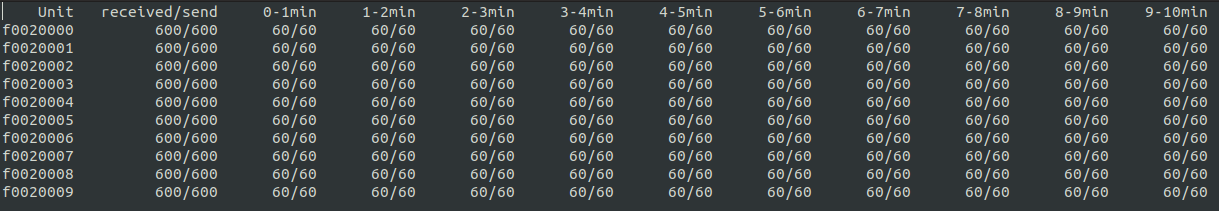
\includegraphics{obrazky-figures/output_test.png}
    }
  \caption{Ukázka výstupu vyhodnocovacího skriptu.}\label{pic:load_verif_script}
\end{figure}

Pro průběh každého testu bylo nutné vytvořit jednotlivé databáze, což je u~desítek zařízení velmi zdlouhavé. K~přidávání jednotek do databáze pojmenovaných podle pravidla zmíněného dříve byl vytvořen skript \textit{createTestDatabases.sh} umístěný ve stejné složce jako skript vyhodnocovací. Vstupními argumenty jsou počet jednotek \textit{-u <jednotek>} a číslo testu \textit{-t <číslo testu>}. Skript se pokusí před vytvořením databází smazat staré databáze se stejným názvem. 

Výsledky testů bez zabezpečení je možné vidět v~tabulce \ref{tab:graph_test_1}. Sloupec \textit{jednotek} udává počet virtuálních jednotek, \textit{zpoždění} stanovuje dobu mezi zprávami od jedné jednotky, \textit{délka t.} určuje dobu trvání testu, \textit{přijato} určuje v~procentech kolik odeslaných zpráv bylo přijato a \textit{zpráv/s} udává kolik zpráv dohromady UDP server obdržel každou vteřinu. Výstupy všech testů vygenerovaných vyhodnocovacím skriptem jsou na přiloženém médiu ve složce \textit{Testing/output/}. 

Prvních devět testů bylo určeno pro hrubý odhad maximálního limitu zpracovaných zpráv. Z~testů vyplývá, že UDP server zvládá bez problému zpracovat a zapsat do databáze sto zpráv za vteřinu. Při tisíci zprávách za vteřinu docházelo již k~1-4\% ztrátám. Při deseti tisících zprávách za vteřinu byla ztrátovost přes 90 \%. Tyto hodnoty naznačují, že maximální množství zpracovaných zpráv na testovaného zařízení je zhruba $950-980$ za vteřinu ze všech jednotek. 

Testy číslo 10, 11 a 12 sloužily k~přesnějšímu určení bezpečného limitu zpracovaných zpráv. Bezpečné množství, při které nedošlo k~žádné ztrátě, je zhruba 600 zpráv za vteřinu. Počet zpráv lze zvýšit zlepšením parametrů zařízení, na kterém je UDP server spouštěn. Je potřeba také brát v~potaz, že na stejném zařízení byla spuštěna i časová databáze. Maximální počet agregovaných hodnot, které je jednotka schopná vygenerovat ve verzi 1.0, je 400 hodnot za vteřinu ze všech senzorů. Jedna UDP zpráva protokolu používaného v~této práci pojme až 56 hodnot. Jednotka je tedy schopná vygenerovat maximálně 8 UDP zpráv za vteřinu. Testovaný UDP server bez zabezpečení zvládne zpracovávat data bez ztráty od 75 jednotek.

Testy 12 a 13 z~tabulky \ref{tab:graph_test_1} byly provedeny se zašifrovanými zprávami. Zprávy byly šifrovány pomocí operace XOR\footnote{https://teambi0s.gitlab.io/bi0s-wiki/crypto/xor/}. Šifrování funguje na principu bitového klíče, který je stejně dlouhý jako UPD zpráva. Klíč zná pouze serverová a klientská aplikace a na jednotku je dodán při její instalaci. Každý bit odesílané zprávy je změněn operací XOR s~odpovídajícím bitem klíče. Zpráva je následně odeslána a na serveru stejným způsobem dekódována. Jak je možné vidět v~tabulce, šifrování mělo vliv na množství zpracovaných zpráv. Už u~600 zpráv docházelo k~drobným výpadkům kolem 0,07 \%, snížení počtu zpráv na 500 za vteřinu tento výpadek vyřešilo.

Pokud by bylo potřebné zpracovávat data od více jednotek, je nutné využít více instancí serveru a program pro vyvažování zátěže testovaný v~\ref{sec:load_balancing}.

\begin{table}[h]
    \begin{center}
        \begin{tabular}{|c|c|c|c|c|c|}
        \hline
             č. testu & jednotek & zpoždění[ms] & délka t.[min]& přijato[\%] & zpráv/s\\ \hline
             $1$ & $1$ & $1000$ & $10$ & $100$ & $1$\\\hline
             $2$ & $10$ & $1000$ & $10$ & $100$ & $10$  \\\hline
             $3$ & $100$ & $1000$ & $10$ & $100$ & $100$  \\\hline
             $4$ & $1$ & $100$ & $10$ & $100$ & $10$  \\\hline
             $5$ & $10$ & $100$ & $10$ & $100$ & $100$ \\\hline
             $6$ & $100$ & $100$ & $10$ & $97,75$ & $1000$  \\\hline
             $7$ & $1$ & $10$ & $10$ & $99,99$ & $100$  \\ \hline
             $8$ & $10$ & $10$ & $10$ & $96,78$ & $1000$  \\ \hline
             $9$ & $100$ & $10$ & $10$ & $8,91$ & $10000$ \\ \hline
             $10$ & $90$ & $100$ & $10$ & $91,98$ & $900$ \\ \hline
             $11$ & $80$ & $100$ & $10$ & $95,85$ & $800$ \\ \hline
             $12$ & $60$ & $100$ & $10$ & $100$ & $600$ \\ \hline \hline
             $13$ & $60$ & $100$ & $10$ & $99,93$ & $600$ \\ \hline
             $14$ & $50$ & $100$ & $10$ & $100$ & $500$ \\ \hline
        \end{tabular}
        \caption{Výsledky zátěžových testů UDP serveru.} \label{tab:graph_test_1}
    \end{center}
\end{table}

\subsection{TCP server}
Pro testování TCP serveru bylo opět využito testovacího programu \textit{MessageGenerator}. Cílem testu bylo zjištění, od kolika jednotek je server schopný přijímat data. Výsledky testů jsou v~tabulce \ref{tab:graph_test_2}. Oproti předchozímu testu přibyl sloupec \textit{interval}, určující jak dlouhý časový úsek měření zpráva obsahuje. Během každého testu byly určitou dobu odesílány zprávy s~fixním zpožděním. K~zahlcení došlo, pokud server po uplynutí určené doby nezpracoval požadovaný počet zpráv. 

Počet maximálního množství jednotek je určen několika faktory. Závisí na délce zprávy, kterou jednotka odesílá, a také jak často tyto zprávy odesílá. TCP protokol a implementace jednotky umožňují jako nejnáročnější možnou kombinaci nastavení zprávy obsahující jednu vteřinu měření odesílané každou vteřinu, tzn. téměř nepřetržitý datový tok od každé jednotky. Toto nastavení by ovšem vedlo k~rychlému zahlcení serverové aplikace a mohlo by způsobit výpadky v~měření. Proto je jako nejhorší možný scénář zvoleno nastavení měření o~délce deseti vteřin a odesílání všech dat. Testy 1, 2, 3 a 4 se zabývají právě touto situací. Z~výsledku lze odvodit, že TCP server je schopný zpracovávat data od 50 jednotek, které posílají veškerá naměřená data po deseti vteřinových úsecích (zhruba pět zpráv za vteřinu). 

Systém ovšem není koncipován na odesílání veškerých naměřených nezpracovaných dat, ale na odesílání intervalů nezpracovaných dat po určitém čase. Testy 5 a 6 vychází ze situace, kdy každá jednotka odesílá desetivteřinové úseky měření jednou za minutu. Podle dosavadních výsledků by server měl v~této situaci zvládat zpracovávat data až od 300 jednotek a test číslo 5 to potvrzuje.

\begin{table}[h]
    \begin{center}
        \begin{tabular}{|c|c|c|c|c|c|c|}
        \hline
             č. testu & jednotek & zpoždění[s] & délka t.[min] & interval[s] &  přijato[\%] & zpráv/s\\ \hline
             $1$ & $10$ & $10$ & $5$ & $10$ & $100$ & $1$  \\\hline
             $2$ & $100$ & $10$ & $5$ & $10$ & $59,1$ & $10$  \\\hline
             $3$ & $50$ & $10$ & $5$ & $10$ & $100$ & $5$  \\\hline
             $4$ & $70$ & $10$ & $5$ & $10$ & $83,62$ & $7$  \\\hline
             $5$ & $300$ & $60$ & $10$ & $10$ & $100$ & $5$  \\\hline
             $6$ & $300$ & $60$ & $10$ & $10$ & $100$ & $5$  \\\hline
        \end{tabular}
        \caption{Výsledky zátěžových testů TCP serveru.} \label{tab:graph_test_2}
    \end{center}
\end{table}
Další test byl proveden se zabezpečenou komunikací. Spojení bylo zabezpečeno pomocí knihovny open-ssl a k~implementaci byl využit příklad z~\cite{openssl}. Klíč vygenerovaný k~tomuto testu je umístěn na přiloženém médiu v~kořenovém adresáři. Z~testu vyplývá, že zabezpečení spojení nemělo vliv na maximální počet zpracovaných zpráv.

Při testování TCP serveru bylo zjištěno, že je schopný bez zahlcení zpracovávat 5 zpráv za vteřinu obsahující desetivteřinová měření. Počet jednotek, od kterých je schopný data zpracovávat, záleží na jejich nastavení. Při odesílání dat každou minutu je schopný zpracovávat data až od 300 jednotek, což je mnohem více, než je schopný zpracovávat UDP server.

\section{Škálovatelnost} \label{sec:load_balancing}
Jak již bylo prokázáno v~předchozích testech, celý systém může být spuštěn na jednom zařízení s~limitem zhruba 75 jednotek bez zabezpečené komunikace a 65 jednotek se zabezpečenou komunikací. Při nutnosti obsluhy více jednotek je nutné systém škálovat. Škálovatelnost serverové části se dělí na dvě oblasti -- zpracování dat a úložiště. 

Škálování úložiště se odvíjí od zvoleného řešení. V~případě testované časové databáze InfluxDB lze využít placenou verzi, schopnou distribuovat data mezi více uzlů\footnote{https://www.influxdata.com/blog/influxdb-clustering/}.

Množství dat zpracovaných UDP a TCP serverem lze zvýšit spuštěním více instancí těchto programů na více uzlech a jejich rovnoměrným vytížením. Rozložit vytížení (anglicky \textit{Load balancing}) lze pomocí hardwarového zařízení nebo softwaru. Pro tento test byl zvolen program \textit{pen}\footnote{https://github.com/UlricE/pen}. Program byl spuštěn s~parametry \textit{pen -r -U 9944 127.0.0.1:9943 192.168.1.28:9943}. UDP zprávy přijímané na portu 9944 byly tedy distribuovány mezi dvě zařízení na port 9943. Výsledky testu je možné vidět v~tabulce \ref{tab:graph_test_3}. Testy systému s~více instancemi UDP serveru na více zařízeních prokázaly, že došlo ke zvýšení limitu počtu zpracovávaných zpráv. V~testu číslo 1,2 a 3 byla využita tři zařízení. První zařízení generovalo zprávy, druhé zařízení provádělo zpracování poloviny zpráv a přeposílalo druhou polovinu třetímu zařízení, které provádělo zpracování druhé poloviny a byla na něm spuštěna databáze. V~těchto testech došlo k~téměř zdvojnásobení počtu zpracovaných zpráv.
Ideální stav je, když každá část systému má své dedikované zařízení. To znamená, že je v~systému zařízení sloužící pouze k~rozložení zatížení, několik zařízení pouze pro příjem zpráv a další pouze s~databázovými uzly.

\begin{table}[h]
    \begin{center}
        \begin{tabular}{|c|c|c|c|c|c|}
        \hline
             č. testu & jednotek & zpoždění[ms] & délka t.[min]& přijato[\%] & zpráv/s\\ \hline
             $1$ & $100$ & $50$ & $10$ & $69.63$ & $2000$\\\hline
             $2$ & $50$ & $50$ & $10$ & $100$ & $1000$  \\\hline
             $3$ & $70$ & $50$ & $10$ & $98.65$ & $1400$  \\\hline
        \end{tabular}
        \caption{Výsledky zátěžových testů UDP s~rozložením vytížení.} \label{tab:graph_test_3}
    \end{center}
\end{table}

\begin{figure}[h]
  \centering
  \scalebox{0.20}{
        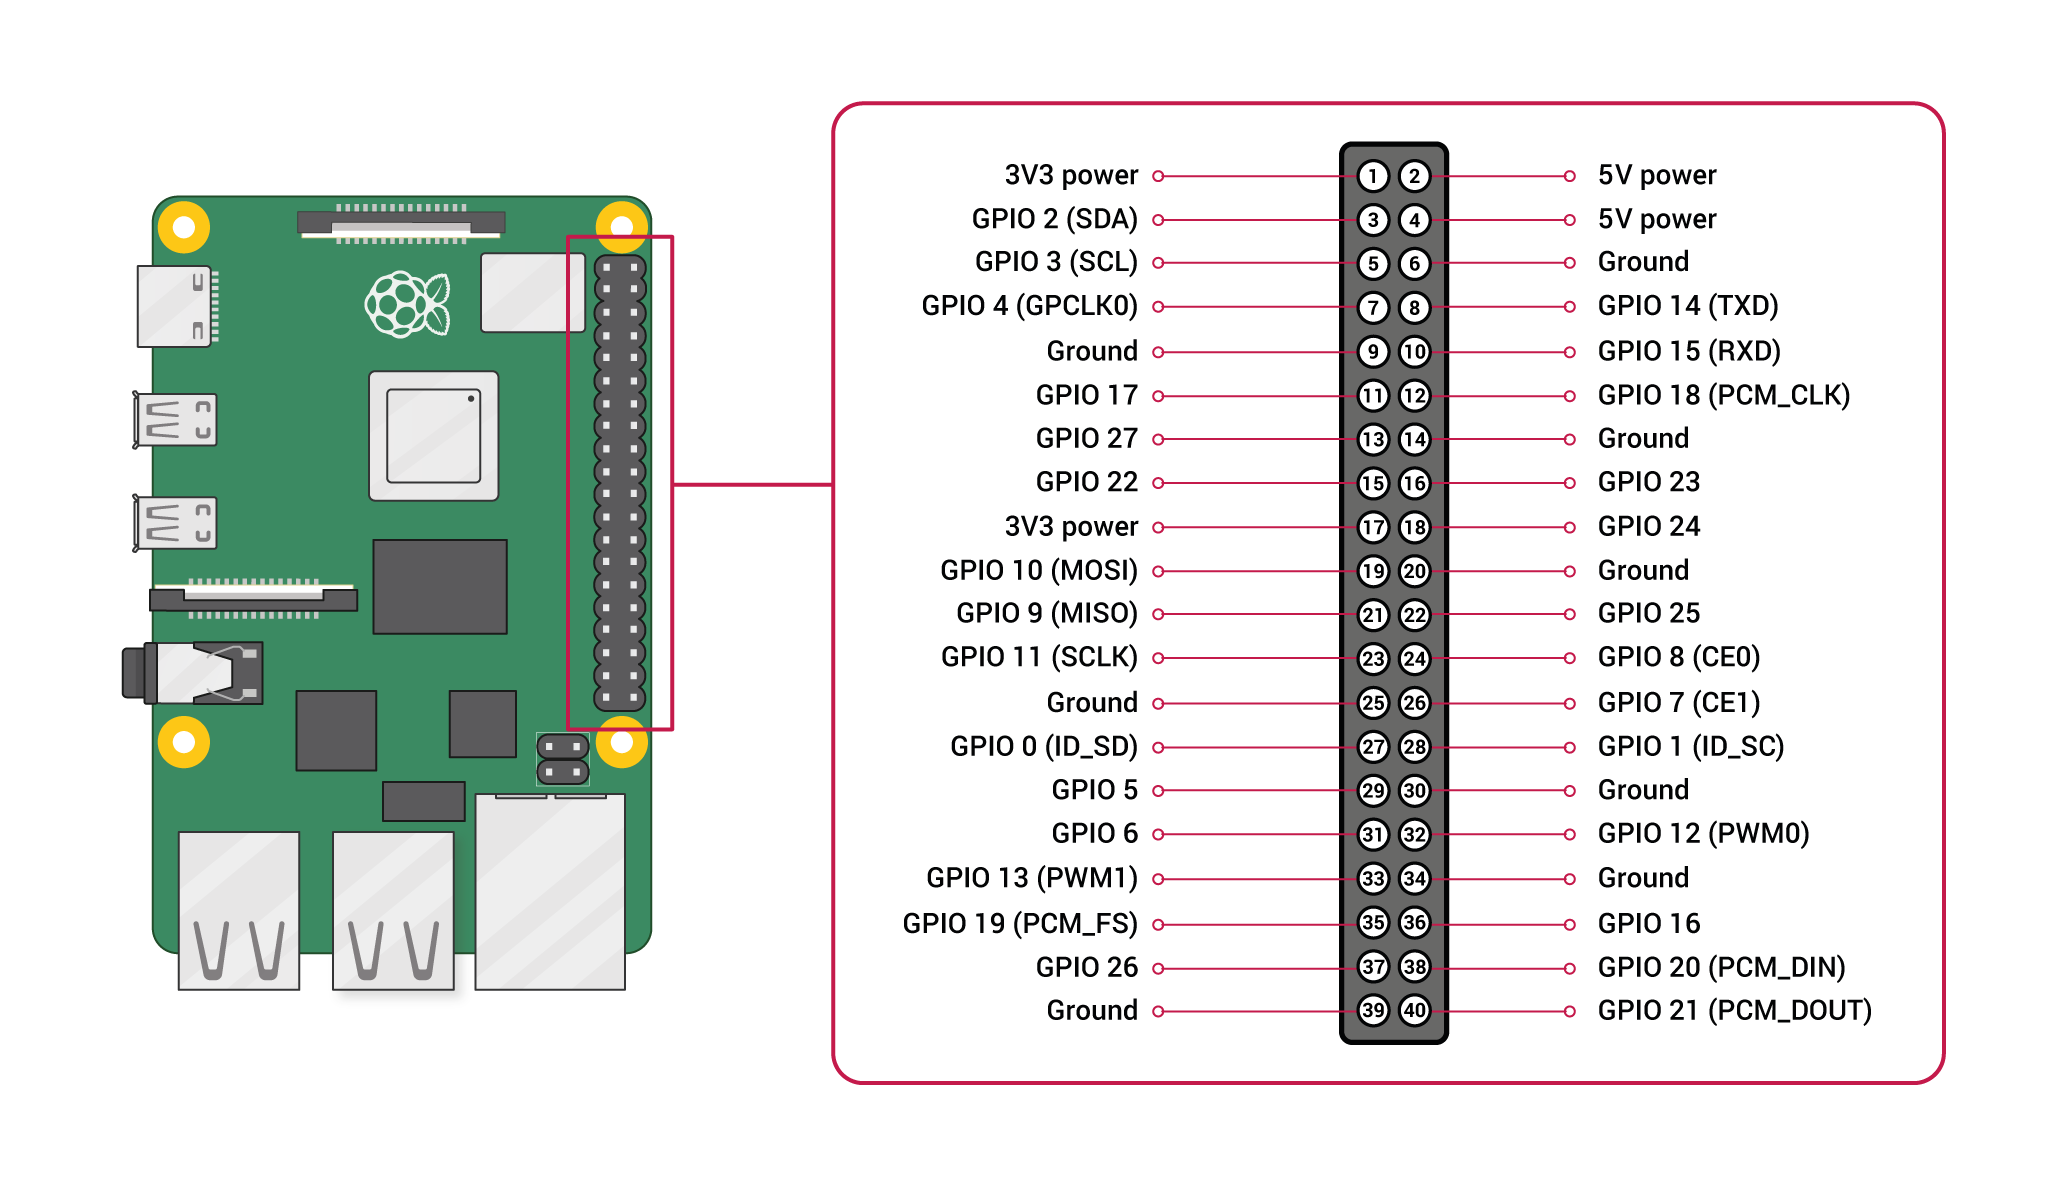
\includegraphics{obrazky-figures/gpio.png}
    }
  \caption{Rozložení pinů na Raspberry Pi \cite{rpi_doku}.}\label{pic:gpio_pinout}
\end{figure}

\section{Měření jednotky}
Cílem tohoto testu bylo ověřit, zda RPi vyčítá data o~správné vzorkovací rychlosti z~rozšiřující desky nebo souboru a nedochází ke ztrátě dat. Pokud jednotka čte data ze souboru, je vyveden hodinový signál o~nastavené frekvenci na jeden z~GPIO pinů a tento pin je fyzicky propojen s~pinem nastaveným jako \textit{data ready}. Výstupní frekvence výstupního pinu byla změřena pomocí osciloskopu. Na obrázku \ref{pic:gpio_pinout} je možné vidět rozložení pinů na RPi. Sonda byla připojena k~vývodu hodinového signálu na pinu číslo 7 (GPCLK0). Frekvence výstupního signálu byla nastavena na 128 kHz a souhlasila s~hodnotou odečtenou na osciloskopu. Rychlost čtení z~rozhraní SPI byla také ověřována pomocí osciloskopu. K~RPi s~připojenou rozšiřující deskou byly připojeny dvě sondy. Prví sonda byla připojena k~pinu číslo 15 (GPIO 22), na který je přiváděn signál \textit{data ready}. Druhá sonda byla připojena na pin číslo 21 (GPIO 9), který funguje jako MISO (Master In Slave Out -- příchozí data z~SPI od rozšiřující desky). Komunikace byla zaznamenána nejdříve při vzorkovací frekvenci 64 kHz a posléze i při frekvenci 128 kHz. Část komunikace mezi deskou a RPi z~prvního testu je možné vidět na obrázku \ref{pic:osciloscop}.

\begin{figure}[h]
  \centering
  \scalebox{0.22}{
        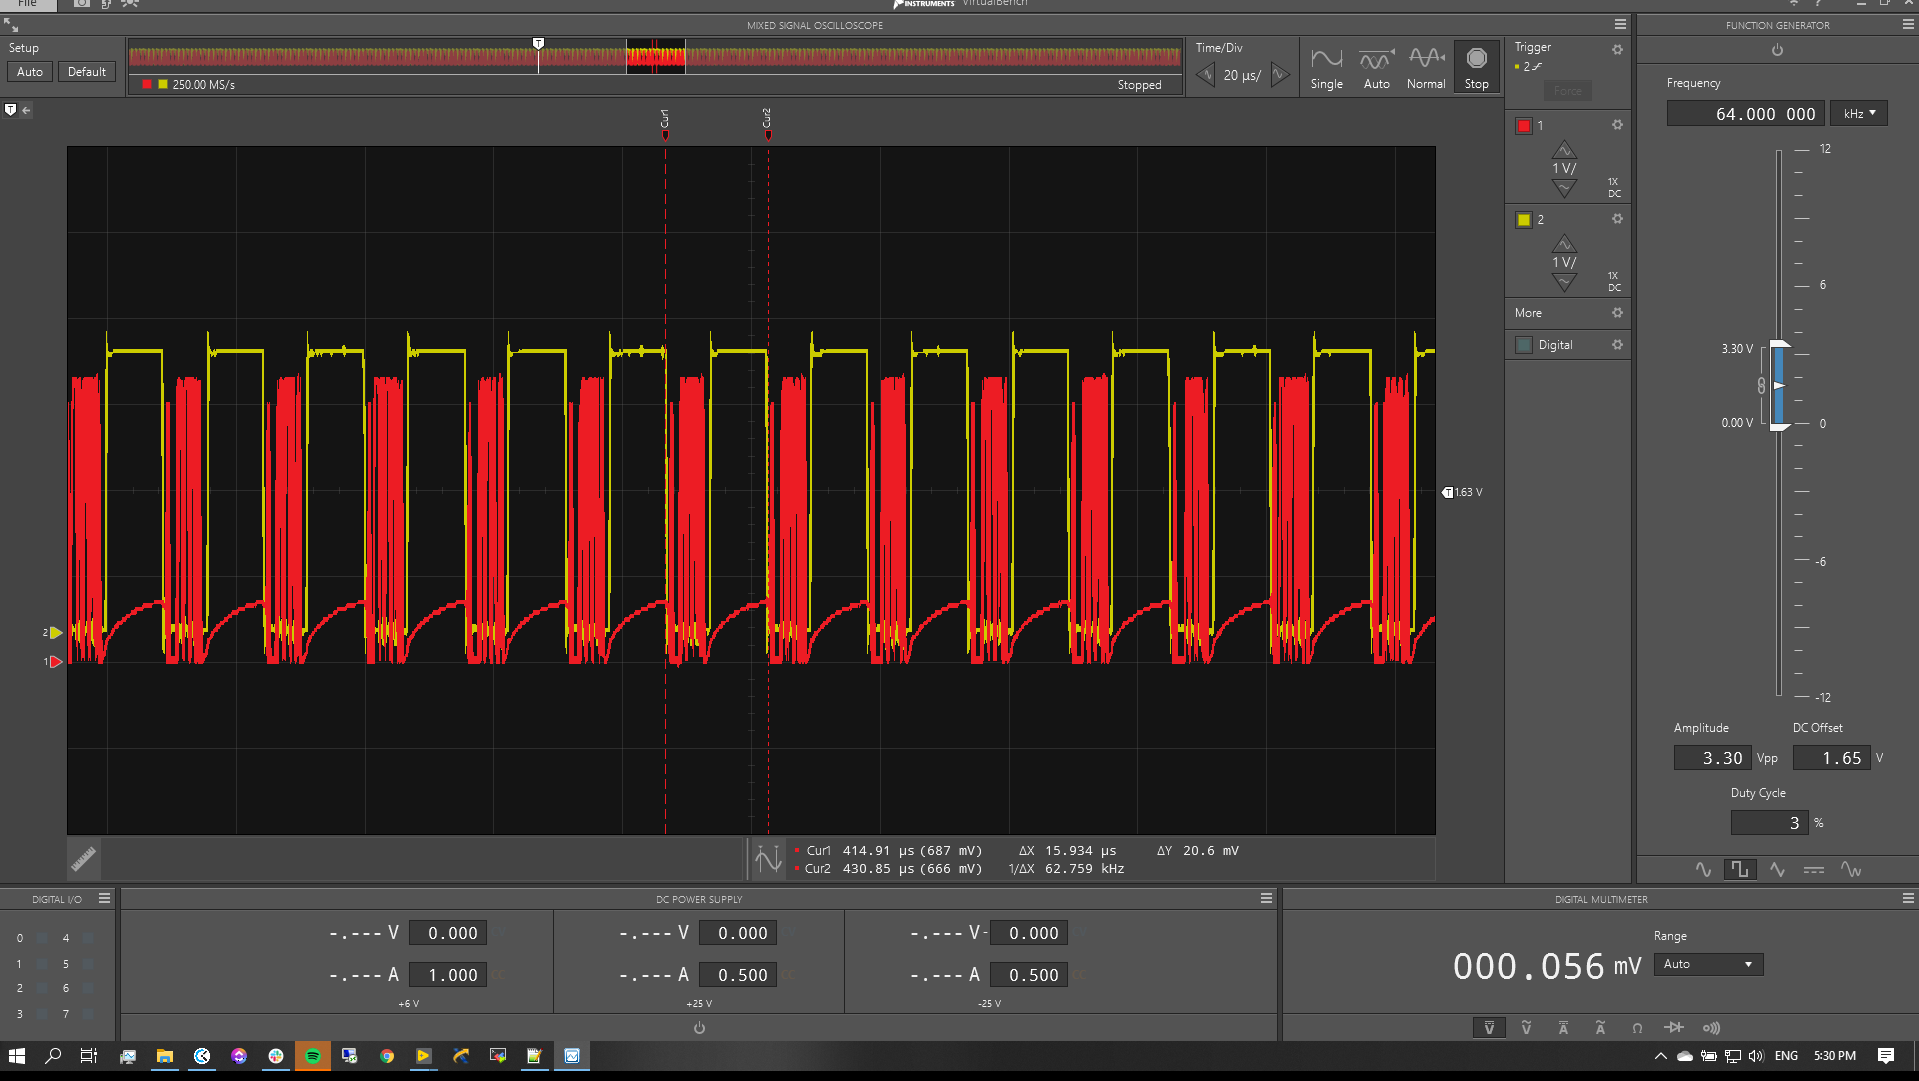
\includegraphics{obrazky-figures/osciloskop64kHz.png}
    }
  \caption{Komunikace přes SPI při 64 kHz mezi RPi a rozšiřující deskou.}\label{pic:osciloscop}
\end{figure}

Na obrázku je možné vidět žlutě značený signál \textit{data ready}. Signál má skutečně frekvenci 64 kHz, nastavení AD převodníku tudíž proběhlo správně. Červeně značený signál značí čtení dat z~převodníku. Data jsou čtena při sestupné hraně signálu \textit{data ready}. V~měření nebylo jediné vynechání čtení. Z~obrázku je patrné, že RPi strávilo čtením dat méně než polovinu doby před příchodem další sestupné hrany. Stejným způsobem bylo změřeno i čtení dat o~vzorkovací frekvenci 128 kHz. Stejně jako při předchozím testu nedocházelo k~vynechání dat, zařízení využívalo zhruba 90 \% času mezi jednotlivými sestupnými hranami pro čtení. Vyšší vzorkovací frekvenci by testovaná implementace nestíhala číst.

\section{Detekce překročení limitu s~historickými daty}
Cílem testu bylo ověřit sledování příchozích dat do databáze a upozornění na překročení limitu u~senzoru. K~testu byla využita historická agregovaná data partnerské firmy obsahující poruchu stroje. Data byla obdržena ve formátu csv. Pro účely testu byl vytvořen program \textit{CSVImport}, umístěný na přiloženém médiu ve složce \textit{Testing/}. Vstupními argumenty jsou \textit{-f <soubor>} s~názvem souboru, který má být importován, \textit{-a <ipv4>} adresa serveru a \textit{-p <port>} s~portem cílového serveru. Program postupně čte hodnoty ze souboru a vytváří UDP zprávy, které odesílá UDP serveru. Pro tento test nemohlo být využito čtení ze souboru na jednotce, protože byly poskytnuty již agregované hodnoty a implementace čtení ze souboru na jednotce vyžaduje nezpracovaná data o~nastavené vzorkovací frekvenci. Csv soubor \textit{data.csv}, použitý k~tomuto testu, je umístěn na přiloženém médiu v~kořenovém adresáři. Každý řádek souboru obsahuje unixovou časovou značku v~milisekundách a naměřenou hodnotu.

K~detekci překonání nastaveného limitu hodnoty bylo využito nástroje Kapacitor, dostupného s~databází InfluxDB. Při instalaci nástroje bylo postupováno podle dokumentace\footnote{https://docs.influxdata.com/kapacitor/v1.5/introduction/installation/}. Po spuštění nástroje je možné ho ovládat přes webové rozhraní Chronograf. Limit poruchy byl u~partnerské firmy nastaven na hodnotu 0.45, pro účely testu byla nastavena stejná hodnota. Jako způsob upozornění o~překročení limitu bylo zvoleno odeslání emailu. Data byla odesílána po jedné vteřině a okamžitě po překročení nastaveného limitu byl odeslán email s~přednastavenou zprávou na zvolenou emailovou adresu. Stránku pro správu upozornění i s~překročenou hodnotou je možné vidět na obrázku \ref{pic:alert}. 

Test prokázal schopnost implementovaného systému upozornit uživatele při překročení nastaveného limitu jednotky. 

\begin{figure}[h]
  \centering
  \scalebox{0.22}{
        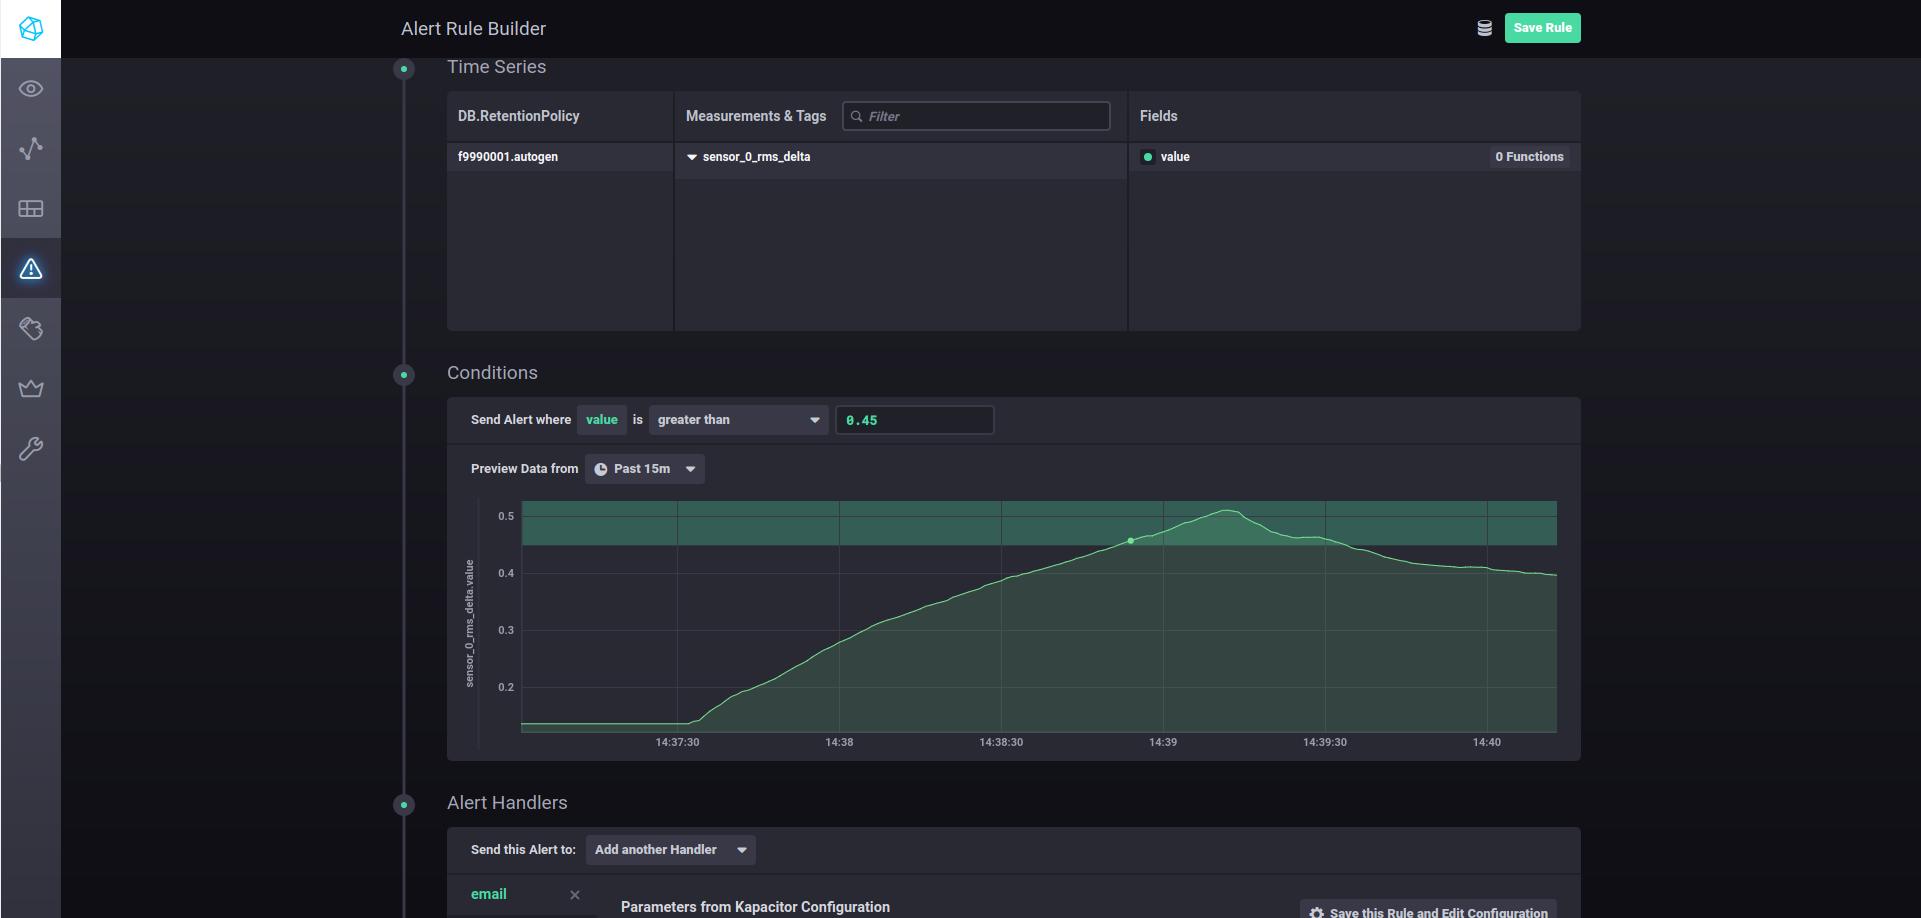
\includegraphics{obrazky-figures/alert.png}
    }
  \caption{Správa pravidla pro Kapacitor v~aplikaci Chronograf.}\label{pic:alert}
\end{figure}

